%%%%%%%%%%%%%%%%%%%%%%%%%%%%%% -*- Mode: Latex -*- %%%%%%%%%%%%%%%%%%%%%%%%%%%%
%% 04-14.tex -- Thesis white paper - software inspections
%% Author          : Aaron A. Kagawa
%% Created On      : Mon Sep 23 11:52:28 2004
%% Last Modified By: Aaron Kagawa
%% Last Modified On: Sat Nov 20 13:21:38 2004
%% RCS: $Id$
%%%%%%%%%%%%%%%%%%%%%%%%%%%%%%%%%%%%%%%%%%%%%%%%%%%%%%%%%%%%%%%%%%%%%%%%%%%%%%
%%   Copyright (C) 2004 Aaron A. Kagawa
%%%%%%%%%%%%%%%%%%%%%%%%%%%%%%%%%%%%%%%%%%%%%%%%%%%%%%%%%%%%%%%%%%%%%%%%%%%%%%%
%% 

\documentclass[11pt,twocolumn]{article} 
\input{/export/home/csdl/tex/psfig/psfig}
\usepackage{/export/home/csdl/tex/icse2003/latex8}
\usepackage{times}
%% A verbatim-like environment which allows font changes
%%\usepackage{alltt}
%% New LaTeX2e graphics support
\usepackage[final]{graphicx}
% uncomment the % away on next line to produce the final camera-ready version
% and uncomment the \thispagestyle{empty} following \maketitle
\pagestyle{empty}

\begin{document}

\title{Limited Resource Software Inspections}

\author{\protect\begin{tabular}{ccc}
Aaron A. Kagawa \\
\end{tabular}\\
\em  Collaborative Software Development Laboratory \\
\em  Department of Information and Computer Sciences \\
\em  University of Hawai'i \\
\em  Honolulu, HI 96822 \\
\em  kagawaa@hawaii.edu}
\maketitle
\thispagestyle{empty}

\begin{abstract}  % 200 words
Imagine that your project manager has budgeted 200 person-hours for the
next month to inspect newly created source code.  Unfortunately, in order
to inspect all of the documents adequately, you estimate that it will
take 400 person-hours.  However, your manager refuses to increase the
budgeted resources for the inspections.  How do you decide
which documents to inspect and which documents to skip?

The classic definition of Inspection, does not provide any advice on how to
handle this situation. For example, the notion of entry criteria used in
Software Inspection determines when documents are ready for inspection
rather than if inspection is needed at all \cite{Ebenau94}.

%% I could talk about previous approaches here. Sampling and Up-Stream documents

This proposed research will investigate how to prioritize inspection
resources and apply them to areas of the system that need them the most.
It is commonly assumed that defects are not uniformly distributed across
all documents in a system - that a relatively small subset of a system
accounts for a relatively large proportion of defects \cite{Boehm01}.  If
inspection resources are limited, then it will be most effective to
identify and inspect the defect-prone areas.

To accomplish this research, I will construct an evaluation framework based
upon automated process and product measures to distinguish documents that
are in ``most need of inspection'' from those in ``least need of
inspection''.  Some examples of the process and product measures that are
being considered include: reported defects, unit tests, test coverage,
active time, and number of changes. Based on this framework I hypothesize,
that code deemed in most need of inspection will generate more critical
issues than code deemed least need of inspection.

%% Each measure acts as an indedendent variable for determining the inspection
%% candidacy of a document and can be assigned an individual weight. 

Each measure affects the determination of ``most and least'' differently.
For example, suppose that test coverage should be weighted more than active
time. Therefore, weights of each measure will be calibrated based on my
initial guesses.  My research will employ a very simple evaluation
strategy, which includes selecting code to inspect, analyzing the results,
and adjusting the calibration of the measures.

There are three milestones that measure my progress in this reasearch.
Milestone 1: implementation of Hackystat Extension, January 2005.
Milestone 2: completed evaluation, March 2005. Milestone 3: thesis
submission and defense, April 2005.
\end{abstract}

%%%%%%%%%%%%%%%%%%%%%%%%%%%%% -*- Mode: Latex -*- %%%%%%%%%%%%%%%%%%%%%%%%%%%%
%% 04-14-intro.tex -- Priority Ranked Software Inspection
%% Author          : Aaron A. Kagawa
%% Created On      : Mon Sep 23 11:52:28 2004
%% Last Modified By: Aaron Kagawa
%% Last Modified On: Sat Feb  5 13:25:36 2005
%% RCS: $Id$
%%%%%%%%%%%%%%%%%%%%%%%%%%%%%%%%%%%%%%%%%%%%%%%%%%%%%%%%%%%%%%%%%%%%%%%%%%%%%%
%%   Copyright (C) 2004 Aaron A. Kagawa
%%%%%%%%%%%%%%%%%%%%%%%%%%%%%%%%%%%%%%%%%%%%%%%%%%%%%%%%%%%%%%%%%%%%%%%%%%%%%%%


\chapter{Introduction}
Software inspection is defined as: ``A formal evaluation technique in which
software requirements, design, or code are examined in detail by a person
or group other than the author to detect faults, violations of development
standards, and other problems...'' \cite{Gilb93}. Software inspection, or
software review as it is sometimes called, can have fantastic results:
``Rigorous inspection can remove up to 90 percent of errors from a software
product before the fist test case is run'' \cite{Glass03, Bush90}.

Since Michael Fagan invented the inspection technique in 1976, there have
been many variations on the general concept of inspection. We now have
Fagan Inspection \cite{Fagan76}, Software Inspection \cite{Gilb93},
High-Impact Inspection, Phased Inspection, ``regular'' software inspection,
software reviews, code walkthroughs, inspections without meetings, and many
more different twists on the original concept.  Each of these techniques
claim to be the best inspection method for their certain circumstances. For
example, some argue that the inspection meeting is a waste of time and
resources \cite{Johnson97, Johnson98, Votta93}. Others argue that the
inspection meeting is critical for supporting social and educational
aspects of inspection \cite{Johnson98}.

My research is different from traditional inspection research. Instead of
asking how to conduct the inspection process, I ask how to determine what
to inspect, when to conduct inspections, and more importantly if inspection
is really needed for a particular piece of code. In this proposal, I will
describe how the selection of a document for inspection can create problems
for organizations with limited inspection resources. I will then propose a
new inspection document selection technique called Priority Ranked
Inspection and evaluate its effectiveness.


%%Since the introduction of inspections by Michael Fagan, there have been
%%numerous views, descriptions, and process that have been proposed by
%%various authors and researchers. Some of these include; Fagan Inspections
%%\cite{Fagan76}, Software Inspections \cite{Gilb93}, High-Impact
%%Inspections, and Phased Inspections just to name a few. Throughout this
%%paper I will use the lower cased inspection to represent all inspection
%%techniques.

\section{The Problem of Limited Resources for Software Inspections}
The use of software inspection has reported outstanding results in
improving productivity and quality. One study has found that when the
inspection process is followed correctly, up to 95 percent of defects can
be removed before entering the testing phase \cite{Bush90}. In another
success story, the Jet Propulsion Laboratory (JPL) adopted inspection to
identify defects and experienced a savings of 7.5 million dollars by
conducting 300 inspections \cite{Bush90a}. This statistic is very
impressive. However, what is not emphasized is each inspection had an
average total cost of 28 hours. Using that average cost, the total cost for
JPL's inspection process was 8,400 hours or roughly 4 years of work.

The JPL experience illustrates a fundamental problem with inspections:
better results come from substantial investment \cite{Gilb93}. Not all
organizations have the time or the money to invest in full or complete
inspections. In most cases, organizations have limited funds or resources
that can be devoted to inspections. For example, a manager may only have
200 hours of a project schedule to allocate towards quality assurance
including inspections. Such organizations must decide how to best utilize
their limited inspection resources. This realistic management of
inspections directly contradicts the classical inspection adage of ``when a
document is ready, you should inspect it''. The bottom line is that most
organizations cannot inspect every document.

The traditional inspection process begins with the initiation phase, or
sometimes called the planning stage, in which authors volunteer their
documents for inspection \cite {Gilb93}. A inspection leader checks the
document against entry criteria to determine if the document is ready for
inspection \cite{Ebenau94, Gilb93}. Again this process works very well for
organizations, like JPL, that have the resources to inspect every document
after every significant change. However, I believe that this phase of
inspection is a major problem for organizations that do not have the
necessary resources, because the process does not consider that some
documents are ``better'' to inspect than others. A simple illustration of
this fact is that 80 percent of defects come from 20 percent of the system
\cite{Boehm01}.  Thus, volunteering a document from the defect-prone 20
percent will likely be ``more in need of inspection'' than any other part
of the system.

Furthermore, the current literature \cite{Ebenau94, Wiegers02, Gilb93} on
inspections does not provide specific insights into the trade-offs between
inspecting some documents and not inspecting others.  However, Tom Gilb and
Dorothy Graham provide two recommendations to use when inspection resources
are limited; sampling and emphasizing up-stream documents \cite{Gilb93}.
The use of sampling involves inspecting various areas of a system to
identify areas of interest. Up-stream documents are documents that define
high-level requirements or designs.  Inspecting up-stream documents ensures
that the requirements are correct before any implementation is started.
Although, these are very useful recommendations, they do not provide much
specific guidance of how best to use limited inspection resources.

%%For example, consider the following scenario:
%%\begin{quotation}
%%  \textit{The FooBar organization has enough resources available to conduct
%%    two inspections a week. However, this organization creates and finishes
%%    10 different documents each week. How do they select 2 documents from
%%    the possible 10 to inspect? To be fair to all developers they use a
%%    round-robin type approach by allowing a different developer to
%%    volunteer a document for inspection. This approach is fairly successful
%%    and at least they are conducting inspections. But, are they inspecting
%%    the right documents? Obviously, this organization is unavoidably
%%    letting 8 documents slip through the inspection-crack and could be
%%    releasing documents that have critical defects.}
%%\end{quotation}


\section{The Priority Ranked Inspection Approach}
To address some of the problems associated with conducting inspections with
limited resources, I propose a new inspection process called ``Priority
Ranked Inspection'', (PRI). The primary goal of PRI is to optimize the
selection of documents for inspection by distingushing what documents are
``more in need of inspection'' (MINI) versus documents that are ``less in
need of inspection'' (LINI). In addition, PRI will rank each document
according to this determination in hopes of prioritizing the documents that
need to be inspected. The converse is also true: PRI will identify
documents that might not need to be inspected.

As I have shown in the previous section, it is extremely difficult for
organizations with limited inspection resources to inspect every document
before it exits the development process. Therefore, unlike traditional
inspection process, PRI does not require that all documents be inspected.
Instead, PRI is intended to help these organizations in two ways. First,
PRI is intended to be able to identify documents in the current development
process that need to be inspected. This will allow organizations to make an
educated guess at what documents need to be inspected and what documents
can be skipped. Second, it is unavoidable that some documents with critical
defects will finish the development process without being inspected.
Therefore, PRI is also intended to identify documents for inspection
regardless if a document is currently in the development process or not.

%%In the same ways that Software Inspection \cite{Gilb93} is an inspection
%%process, Priority Ranked Inspection is also an inspection
%%process. However, the differences between the two inspection processes lie
%%in the recognition that not all organizations have the necessary resources 
%%to inspect everything. Therefore, PRI is tailored to the organizations with 
%%limited resources. 

There are four primary steps in the Priority Ranked Inspection (PRI)
process. The following list is short description of each of the steps. The
following sub-sections provide a summary description of each step.

\begin{enumerate}
\item The creation of the PRI weighting function, which distinguishes
  MINI documents from LINI documents. The weighting function design
  includes two steps: 
\begin{enumerate}
\item Selection of product and process measures to use in the PRI
  weighting function.
\item Creation of a numerical weighting system that assigns a weight for
  each measure and the calibration of this weighting system.
\end{enumerate}
\item The selection of a document for inspection based on the PRI
  ranking.
\item The actual inspection of the selected document.
\item Adjustment of product and process measure selection and
  calibration based on the results of the inspection.
\end{enumerate}


\subsection{Step 1a: Selection of Product and Process Measures}
The PRI weighting function which distinguishes MINI documents from LINI
documents will be generated automatically from various product and process
measures. Product measures are usually obtainable from direct analysis of
source code.  For example, lines of code, complexity, and number of
children are a few examples of product measures. On the other hand, process
measures are collected from the actual software development process. The
amount of developer 'effort' and the number of defects are examples of
process measures. One might ask, what specific measures should PRI
consider? The answer: it depends on the specific situation. Different
projects and organizations could have a different set of measures in
defining the optimum PRI weighting function and ranking. Therefore, a major
component of the PRI process is the selection of the measures.

Software quality measures are one example of the type of product and
process measures that could be used in PRI. Software inspection has two
primary goals; increase quality and productivity. For this research I am
primarily concerned with increasing quality. The successful inspection of a
document has two main results: finding defects which, once removed,
increases software quality or not finding defects thus indicating high
software quality. Software quality is vaguely defined as ``the degree to
which software possesses a desired combination of attributes''
\cite{IEEEGlossary83}. Some of the possible measures of quality include:
portability, reliability, efficiency, usability, testability,
understandability, and modifiability \cite{Glass03}. Some other widely
accepted measures of quality include defect density and complexity.
Whatever definition used for quality, inspections aim to increase or
validate the level of quality in software.  Therefore, the same measures of
software quality will also provide good indications of what documents need
inspection. For example, finding documents that have low portability,
reliability, efficiency, usability, testability, understandability, and
modifiability would provide a good indication that the documents are MINI.

Based on the previous example, the quality-specific product and process
measures can be extracted and used in the PRI weighting function. Table
\ref{table:step1a} is an example of the PRI ranking of a software project
that contains three documents.  Presented in the table are the measures and
values that are used in the PRI ranking. Due to constraints of the paper
size, the table presents only a couple of the measures discussed above.
However, any number of measures can be used in the PRI weighting function.

\begin{table}[htbp]
  \caption{Step 1a - Example PRI ranking - After Measure Selection}
  \label{table:step1a}
  \begin{center}
    \begin{tabular}{|l|l|l|l|l|l|l|} \hline
      {\bf Document} & {\bf PRI Ranking} & {\bf Reliability} & 
      {\bf Efficiency} & {\bf Testability} & {\bf ...} \\ \hline
Foo.java & MINI & 3 & 4 & 2 & ...  \\ \hline
Bar.java & LINI & 4 & 2 & 6 & ...  \\ \hline
Baz.java & LINI & 1 & 2 & 3 & ...  \\ \hline
    \end{tabular}
  \end{center}
\end{table}

Table \ref{table:step1a} is an illustration of a fictitious PRI ranking.
See Chapter \ref{chapter:system}: Hackystat PRI Extension for more details
about the exact calculations necessary to create a PRI weighting function
and ranking.


\subsection{Step 1b: Calibration of the Product and Process Measures}
Only selecting what measures to be used in the PRI weighting function is
not adequate, because some measures are more important than others. For
example, an organization may find that testability has a greater positive
impact on the PRI weighting function than efficiency. Therefore, Step 1b of
the PRI process is the calibration of the measures' importance. The
calibration of the measures is based on a numerical weighting system. Each
measure will be assigned a numerical weight and will be individually
calibrated. The numerical weighting system and the calibration creates a
PRI ranking, which provides a priority ranking of the documents.

Using the same example (Table \ref{table:step1a}) from the previous
section, imagine that the organization has found testability to be a
leading indicator in defect prevention. Therefore, the calibration is
adjusted and the values of testability are given a higher weight than the
other measures. This finding changes the PRI weighting function and
ranking. The following table (Table \ref{table:step1b}) shows the new PRI
ranking after the calibration.

\label{table:step1b_trial}
\begin{table}[htbp]
  \caption{Step 1b - Example PRI ranking - After Measure Calibration}
  \label{table:step1b}
  \begin{center}
    \begin{tabular}{|l|l|l|l|l|l|l|} \hline
      {\bf Document} & {\bf PRI Ranking} & {\bf Reliability} & 
      {\bf Efficiency} & {\bf Testability} & {\bf ...} \\ \hline
Bar.java & MINI & 4 & 2 & 6 & ...  \\ \hline
Foo.java & MINI & 3 & 4 & 2 & ...  \\ \hline
Baz.java & LINI & 1 & 2 & 3 & ...  \\ \hline
    \end{tabular}
  \end{center}
\end{table}

Notice that, as a result of the calibration, the PRI ranking for Bar.java
has changed from LINI to MINI. This illustrates that the PRI weighting
function and ranking can be flexible and that it has the pontential to
reflect different development processes within different organizations.


\subsection{Step 2: Selecting a Document for Inspection Based on the PRI
  Ranking} After the PRI weighting function and ranking is in place,
an organization may use PRI to select documents for inspection. To select a
document for inspection they simply consult the PRI ranking and find a MINI
document (a document deemed more in need of inspection). This ranking will
help constrain the number of possible documents that can be considered for
inspection.

For example, in the example presented in Table \ref{table:step1b}, an
organization should select Bar.java for the inspection, because it ranked
the highest of the three documents. During the next inspection meeting,
Foo.java should be inspected. However, Baz.java could be skipped, thus
saving inspection resources.

Using the PRI ranking to select documents for inspection has three primary
benefits. First, it can enhance the selection or the volunteering process
of a document for inspection. Second, it can identify documents for
inspection that a volunteering process typically does not. Third,
inspecting a MINI document will generate more critical defects than
inspecting a LINI document.


\subsection{Step 3: Conducting an Inspection of the Selected Document}
Once the document is selected, a traditional inspection process can begin.
PRI does not have any special processes for this step. An organization can
choose to use any traditional inspection process (i.e., Software
Inspection, Fagan Inspection, In-Process Inspection). In other words, the
PRI process is an outer layer that wraps around an already established
inspection process to enhance the selection of documents.  Therefore, in
this research I will not discuss or evaluate traditional inspection
concepts like; inspection leaders, preparation time, etc.


\subsection{Step 4: Adjustment of the Measure Selection and Calibration}
After the inspection of a document, the results can be used to further
improve the PRI weighting function and ranking. For example, if the PRI
weighting function appears to be incorrect, because it ranked a document as
MINI but no major defects were found, then the PRI weighting function
should be adjusted to classify this document as LINI. This adjustment can
be achieved in two ways. First, one could add more product and process
measures to make the PRI weighting function more robust. Alternatively, one
could calibrate the current measures to refine and correct the PRI
weighting function and ranking.  In either case, an incorrect PRI weighting
function will provide data to help make future PRI weighting functions
better. This process should be an ongoing evolving activity.

For example, consider the example presented with Foo.java, Bar.java, and
Baz.java. If an organization has found results that suggest that efficiency
is a leading indicator of defects, then it should be calibrated with a
higher weight.



\section{The Hackystat PRI Extension}
To successfully use PRI, the determination of MINI and LINI must be
obtainable for a very low cost. In other words, if the weighting function
takes three months to generate, a software project will have long past the
need for those specific recommendations. Therefore, this determination must
be obtained in real-time.

One way of obtaining weighting function values in real-time is through the
use of the Hackystat system. Hackystat is a framework for collecting and
analyzing software product and development process metrics in real-time.
For more information about the Hackystat system see Chapter
\ref{chapter:hackystat}.  For this proposed research, I have created an
extension to the Hackystat system called the Hackystat PRI Extension
(hackyPRI for short). hackyPRI provides a real-time PRI weighting function
and ranking. Figure \ref{fig:intro-WorkspacePRIAnalysis} demonstrates the
PRI weighting function and its ranking for a software project that is
obtainable from the Hackystat PRI Extension.

\begin{figure*}[ht]
  \centering
  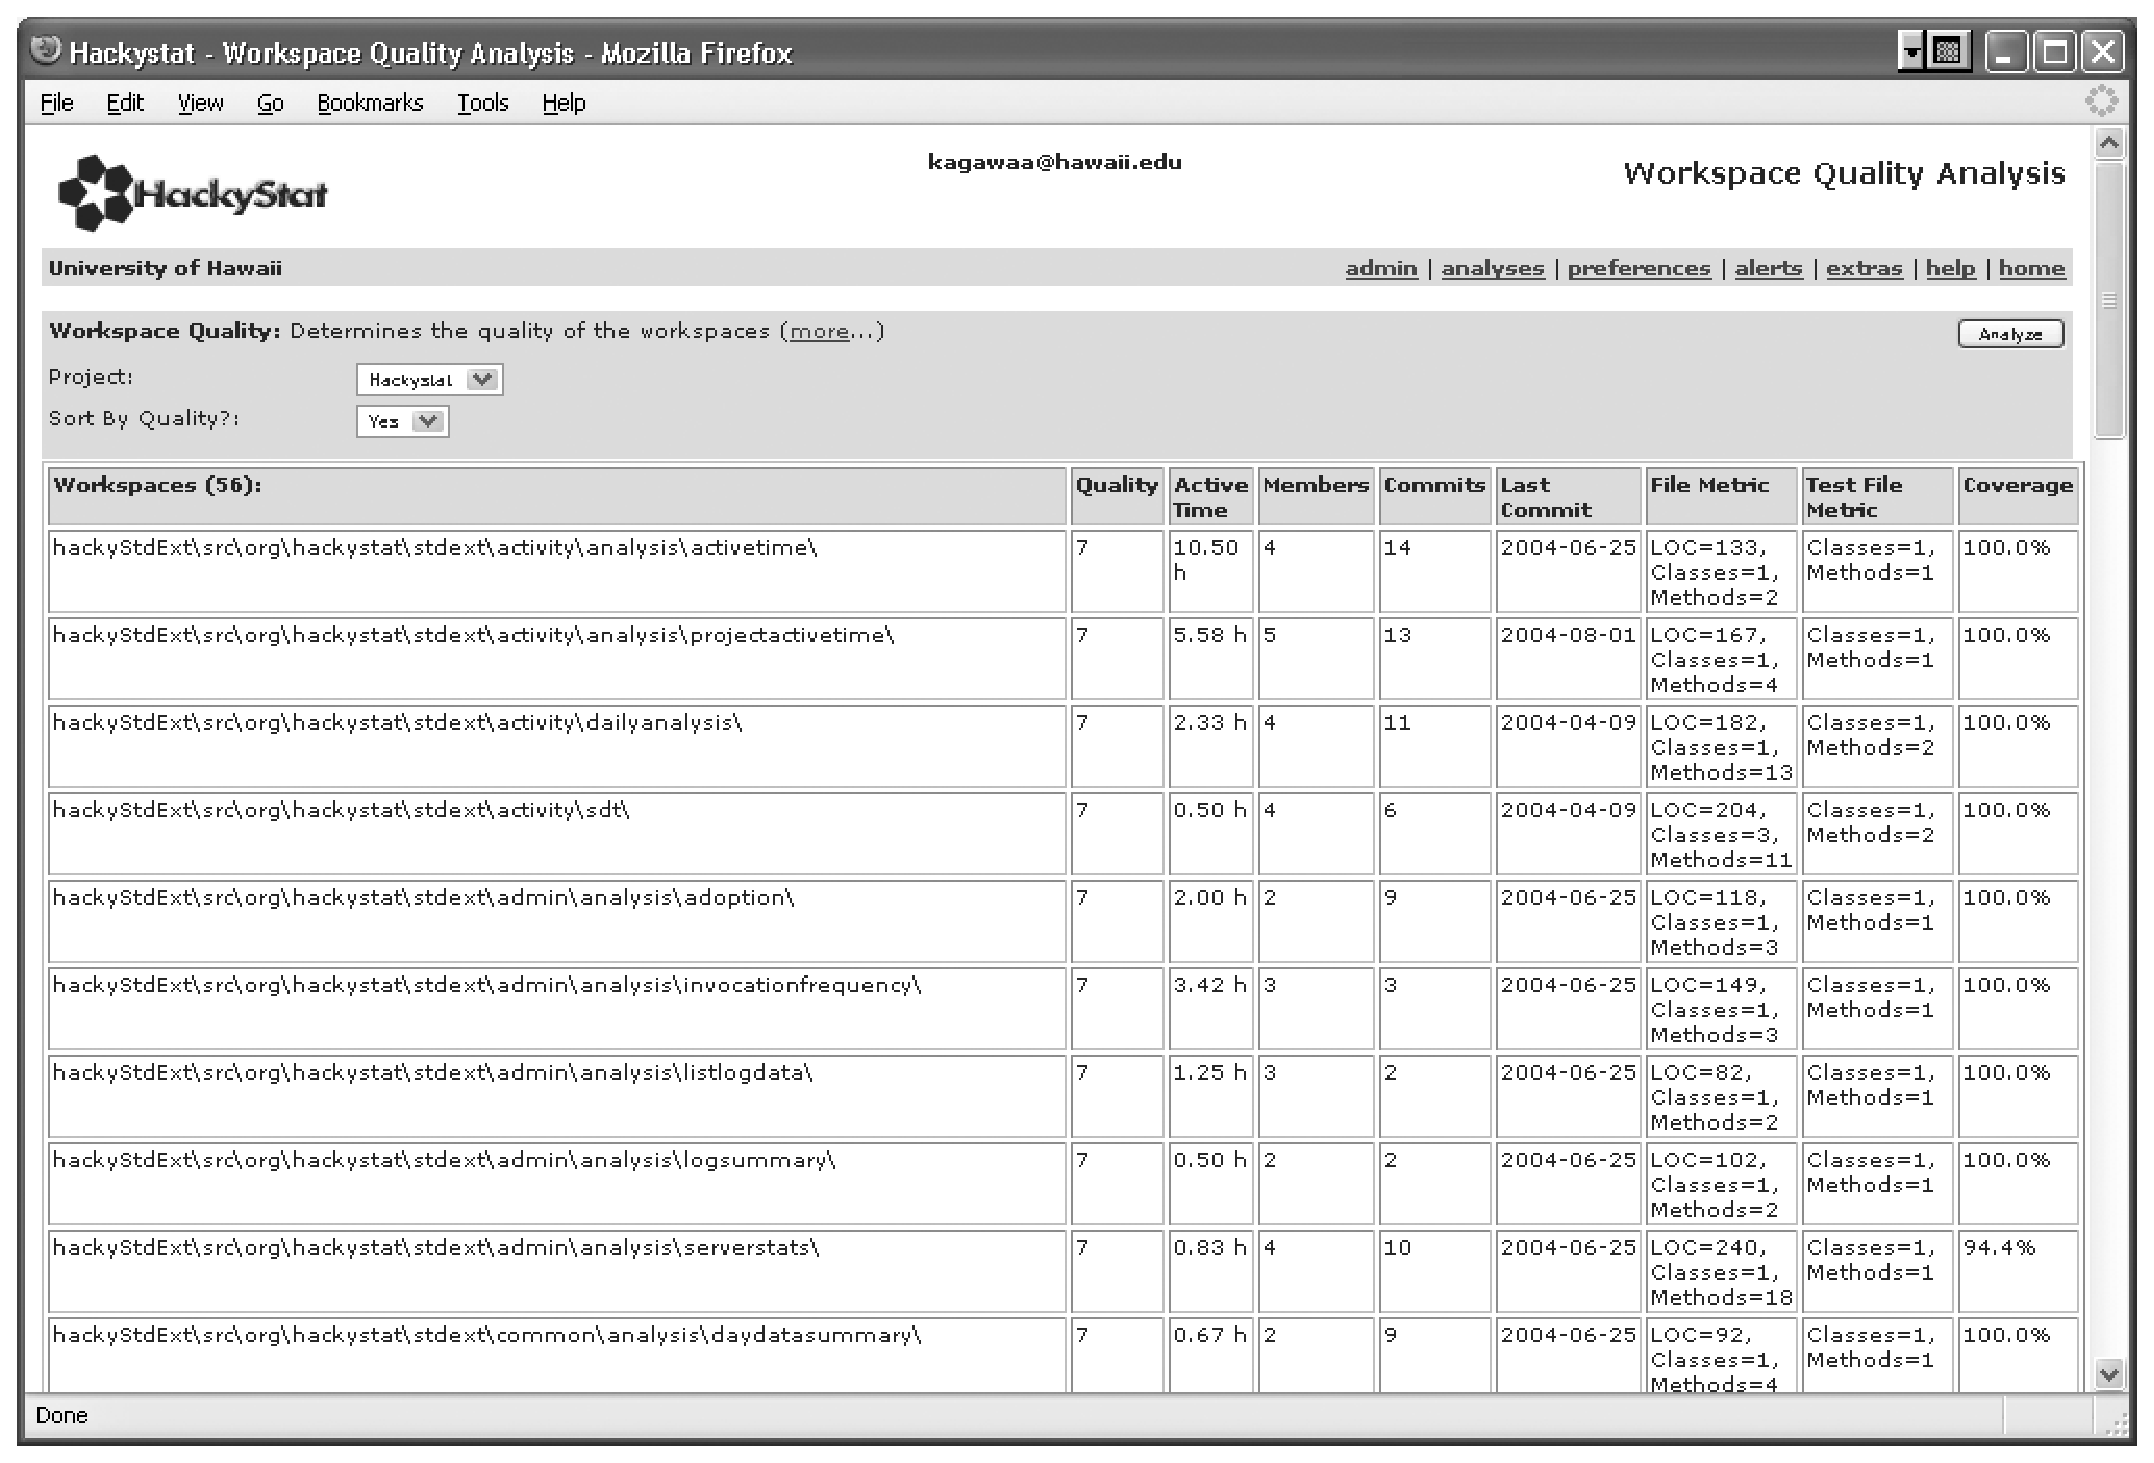
\includegraphics[width=1.00\textwidth]{WorkspaceQuality.eps}
  \caption{The Workspace PRI analysis. Workspaces are listed with its
  respective PRI ranking and measures.}
  \label{fig:intro-WorkspacePRIAnalysis}
\end{figure*}

The Hackystat PRI Extension will be implemented to fully support all 4
steps of the PRI process. The next subsections demonstrate how hackyPRI
supports each of the 4 steps. It is important to note that PRI is a
proposed \textit{process}, therefore many different tools can support it.
Using the Hackystat PRI Extension is not required to conduct PRI
inspections.



\subsection{Step 1a: Selection of Product and Process Measures}
The Hackystat system provides a standard set of product and process
measures, these measures are called Sensor Data Types within the Hacksytat
system, and the means of its collection. Initially, I have developed
hackyPRI to use all of the measures obtainable from Hackystat. In addition,
I have begun to implement a several new Hackystat Sensor Data Types
(measures), that I feel will aid the PRI weighting function.

Each column in Figure \ref{fig:intro-WorkspacePRIAnalysis} is a measure
that is obtainable from Hackystat. Each measure will be automatically and
unobtrusively collected by Hackystat and directly fed in to the hackyPRI
extension.


\subsection{Step 1b: Calibration of Product and Process Measures}
Each measure and its numerical weight will be stored within the hackyPRI
extension. The numerical weights are not shown in Figure
\ref{fig:intro-WorkspacePRIAnalysis}. However, the calibration and
weighting system works behind the scenes to rank each document. For
example, the coverage measure is assigned a numerical weight of 3 if the
coverage value equals 100 percent, 2 if the coverage value is below 90
percent, 1 if the coverage value is below 80 percent, and 0 if the coverage
value is below 70 percent. See Chapter \ref{chapter:system} for a detailed
description about the numerical weighting system.


\subsection{Step 2: Selecting a Document for Inspection Based on the PRI
  Ranking} Using the PRI Hackystat analysis, an organization should
select a document at the bottom of the PRI ranking table for inspection.
The higher the document is in the table, the more it is likely to be LINI.


\subsection{Step 3: Conducting an Inspection of the Selected Document}
Once a document is selected it can be inspected. One interesting side
effect of the PRI ranking is that specific statistics and measures
can be presented during the inspection process. For example, if a document
is selected because it has low coverage, then the inspection can focus on
why the coverage is low.

\subsection{Step 4: Adjustment of the Measure Selection and Calibration}
If a document is shown to be incorrectly ranked, then an adjustment of the
PRI weighting function is necessary. This can be accomplished by adding
more Hackystat measures to the PRI weighting function or recalibrating the
numerical weights associated with the measures. See Chapter
\ref{chapter:system} for a detailed description of the calibration process
for the hackyPRI extension.



\section{Thesis Statement}
The thesis statement of this research is as follows; Priority Ranked
Inspection can distinguish documents that are more in need of inspection
(MINI) from others that need inspection less (LINI). This thesis statement
can be decomposed into the following three main claims, which are based on
the intended benefits of PRI.

\begin{enumerate}
\item PRI can enhance the volunteer-based document selection process.
\item PRI can identify documents that need to be inspected that are not
  typically identified by volunteering.
\item Documents that are deemed more in need of inspection (MINI) will
  generate more critical defects than documents deemed less in need of
  inspection (LINI).
\end{enumerate}

My first claim states that PRI can enhance the selection process. In the
traditional inspection process, this selection process is based on a
developer selecting and volunteering a document for inspection.  This claim
is an intended benefit of PRI because in the traditional inspection process
the number of documents that a developer must select from can vary widely.
If PRI can provide the MINI documents, then the developer can focus his
selection on a smaller set of documents.

My second claim states that PRI can identify documents that have slipped
through the cracks in the development process. For an organization with
limited inspection resources it is not possible to inspect every document.
Therefore, it is inevitable that some documents that need to be inspected
have not been.

My third and last claim states that the inspection of MINI documents will
generate more critical defects than LINI documents. This claim is very
important to the PRI process because if this claim is proven to be false,
then the PRI process cannot solve the limited inspection resource problem.



\section{Evaluation}
This section provides a short description of the methodologies used to
evaluate my thesis claims. Chapter \ref{chapter:evaluation}, Evaluation
Methodology provides a detailed explanation of the methodologies and
procedures that will be used in the evaluation of PRI.

I will evaluate the main thesis of this proposed research by testing each
of my three claims. In this evaluation, I will be studying the inspection
process of the Hackystat system developed by the Collaborative Software
Development Laboratory. I will also be using the developers of Hackystat as
subjects in my evaluation.

My first claim states that PRI enhances the volunteer-based document
selection process. To evaluate this claim, I will conduct a qualitative and
quantitative evaluation.  First, I will assess the developers' current
selection process by asking them to rank a few documents based on what
documents they think are more in need of inspection. Then I will provide
them with the PRI ranking of those same documents and ask them which
rankings would they change. After this qualitative evaluation, I will ask
CSDL to inspect a few documents to evaluate the validity of the developers'
subjective ranking and the PRI ranking.

My second claim states that PRI can identify MINI documents that are not
typically identified by the volunteering process. To evaluate this claim, I
will ask CSDL to inspect a few documents that have not been identified in
the previous evaluation.

My third and last claim states that the inspection of MINI documents will
generate more critical defects than LINI documents. Throughout the
previous two studies I will have collected information about approximately
20 inspections. By quantitatively analyzing the results of these
inspections I will be able to provide supporting evidence for this claim.


\section{Structure of the Proposal}
The remainder of this proposed research is as follows. Chapter
\ref{chapter:relatedwork} discusses previous studies that influenced this
research. Chapter \ref{chapter:hackystat} and Chapter \ref{chapter:system}
contains a detailed description of the Hackystat system and the Priority
Ranked Inspection (PRI) Hackystat extension. Chapter
\ref{chapter:evaluation} discusses the evaluation methodology that will be
implemented to evaluate the claims and benefits of PRI. Chapter
\ref{chapter:contribution} discusses the contributions and future
directions of this research. Finally, Chapter \ref{chapter:timeline}
provides a detailed timeline of this proposed research.














% LocalWords:  Kagawa Sep


%%%%%%%%%%%%%%%%%%%%%%%%%%%%%% -*- Mode: Latex -*- %%%%%%%%%%%%%%%%%%%%%%%%%%%%
%% 04-14.tex -- Thesis white paper - software inspections
%% Author          : Aaron A. Kagawa
%% Created On      : Mon Sep 23 11:52:28 2004
%% Last Modified By: Aaron Kagawa
%% Last Modified On: Tue Nov  9 18:43:00 2004
%% RCS: $Id$
%%%%%%%%%%%%%%%%%%%%%%%%%%%%%%%%%%%%%%%%%%%%%%%%%%%%%%%%%%%%%%%%%%%%%%%%%%%%%%
%%   Copyright (C) 2004 Aaron A. Kagawa
%%%%%%%%%%%%%%%%%%%%%%%%%%%%%%%%%%%%%%%%%%%%%%%%%%%%%%%%%%%%%%%%%%%%%%%%%%%%%%%
%% 

\Section{Related Work}


%%%%%%%%%%%%%%%%%%%%%%%%%%%%%% -*- Mode: Latex -*- %%%%%%%%%%%%%%%%%%%%%%%%%%%%
%% 04-14-system.tex -- Thesis Proposal - PRI
%% Author          : Aaron A. Kagawa
%% Created On      : Mon Sep 23 11:52:28 2004
%% Last Modified By: Aaron Kagawa
%% Last Modified On: Tue Feb  8 21:20:54 2005
%% RCS: $Id$
%%%%%%%%%%%%%%%%%%%%%%%%%%%%%%%%%%%%%%%%%%%%%%%%%%%%%%%%%%%%%%%%%%%%%%%%%%%%%%
%%   Copyright (C) 2004 Aaron A. Kagawa
%%%%%%%%%%%%%%%%%%%%%%%%%%%%%%%%%%%%%%%%%%%%%%%%%%%%%%%%%%%%%%%%%%%%%%%%%%%%%%%

\chapter{Hackystat Priority Ranked Inspection Extension}
\label{chapter:system}
This chapter provides a detailed description of the Hackystat PRI
(hackyPRI) extension. hackyPRI extends the functionality of the Hackystat
system to provide the PRI determination of more and less in need of
inspection (MINI and LINI). I will discuss how hackyPRI supports the four
steps of the Priority Ranked Inspection process.

%%Next, I will provide a detailed description of the design and
%%implementation of the hackyPRI extension.

\section{The Four Steps of the Priority Ranked Inspection Process}
Hackystat PRI Extension supports the four steps of the Priority Ranked
Inspection process. The following list is the four steps of the PRI
process.

\begin{enumerate}
\item The creation of the PRI weighting function, which distinguishes MINI
  documents from LINI documents. The weighting function design includes two 
  steps: 
\begin{enumerate}
\item Selection of product and process measures to use in the PRI
  weighting function.
\item Creation of a numerical weighting system that assigns a weight for
  each measure and the calibration of this weighting system.
\end{enumerate}
\item The selection of a document for inspection based on the PRI
  weighting function and ranking.
\item The actual inspection of the selected document.
\item Adjustment of product and process measure selection and
  calibration based on the results of the inspection.
\end{enumerate}

The following subsections detail how hackyPRI supports the steps.

\subsection{Step 1a: Selection of Product and Process Measures}
The Hackystat system provides a set of Sensor Data Types that represent
various software product and process measures. I will use a subset of the
available Sensor Data Types as the measures that make up the PRI weighting
function. Table \ref{table:measures-hackyPRI} contains a description of the
measures that will be used in the hackyPRI extension.

\begin{table}[htbp]
  \begin{center}
    \caption{Measures used in hackyPRI}
    \label{table:measures-hackyPRI}
    \begin{tabular}{|p{3.0cm}|p{10.0cm}|} \hline
      {\bf Measure} & {\bf Description} \\ \hline
\small{}Expert & \small{}The developer who has the most active time and
commits. An expert represents the developer who is most familiar with the
particular portion of the system. \\ \hline

\small{}Active Time & \small{}The total time developers spent editing a
particular file. This measure is obtainable from attaching Hackystat
sensors to the developers' Integrated Developer Environment (i.e., Emacs,
JBuilder, Eclipse) \\ \hline
\small{}Last Active Time & \small{}The day of the last active time. \\ \hline
\small{}\# of Developer \newline Active Time \newline Contributions &
\small{}The number of unique developers who have contributed to the total
active time. \\ \hline

\small{}Commits & \small{}The total number of commits to a particular
file. This measure is obtainable from attaching Hackystat sensors to a
Concurrent Version Control server (i.e., CVS). \\ \hline
\small{}Last Commit & \small{}The day of the last commit. \\ \hline
\small{}\# of Developer \newline Commit \newline Contributions &
\small{}The number of unique developers who have contributed to the total
commits. \\ \hline

\small{}Review & \small{}The number of code reviews (inspections) that were
conducted. This measure is obtainable from attaching Hackystat sensors
to the Eclipse Jupiter Review plugin.\\ \hline
\small{}Last Review & \small{}The day of the last review or inspection. \\ \hline  

\small{}Defects & \small{}The number of defects that were reported and
stored in the Defect Tracking tool. This measure is obtainable from
attaching Hackystat sensors to the Jira tool.\\ \hline
\small{}Last Defect & \small{}The day of the last defect. \\ \hline

\small{}Enhancements & \small{}The number of enhancements that are
requested. This measure is obtainable from attaching Hackystat sensors to
the Jira tool.\\ \hline
\small{}Last Enhancement & \small{}The day of the last enhancement. \\ \hline

\small{}File Metrics & \small{}The last known metrics of non-test code;
lines of code, number of methods, and number of classes. This measure is
obtainable from attaching Hackystat sensors to the LOCC tool. \\ \hline
\small{}Test File Metrics & \small{}The lines of test code, number of test
methods, and the number of test classes. This measure is obtainable from
the Hackystat sensors to the LOCC tool. \\ \hline

\small{}Dependency & \small{}The inbound and outbound references that
indicate dependencies within the system. This measure is obtainable
from attaching Hackystat sensors to the DependencyFinder tool.\\ \hline

\small{}Unit Tests & \small{}The number of unit tests that are executed
during the last build of the system. This measure is obtainable from
attaching Hackystat sensors to the JUnit tool. \\ \hline 

\small{}Test Failures & \small{}The total number of test failures. This
measure is obtainable from attaching Hackystat sensors to the JUnit
tool. \\ \hline

\small{}Coverage & \small{}The last know coverage percentage of the
system. This measure represents the number of methods that are executed
during a test invocation over the number of total methods. This measure is
obtainable from attaching Hackystat sensors to the JBlanket tool.. \\ \hline

    \end{tabular}
  \end{center}
\end{table}

Each measure is collected for each package or workspace within a specified
project. Figure \ref{fig:WorkspaceQualityAnalysis} shows several example
LINI packages.

\begin{figure*}[ht]
  \centering
  \includegraphics[width=1.00\textwidth]{figs/2004-12-01-all_Page_01.eps}
  \caption{The Workspace PRI analysis. Workspaces are listed with its
  respective PRI ranking and the measures.
}
  \label{fig:WorkspaceQualityAnalysis}
\end{figure*}


\subsection{Step 1b: Calibration of Product and Process Measures}
Each measure and its numerical weight will be stored within the hackyPRI
extension. The numerical weights are not shown in Figure
\ref{fig:WorkspaceQualityAnalysis}, however the calibration and weighting
system works behind the scenes. 

To make the important distinction of MINI and LINI, I assign certain
numerical weights to the measures. For example, if the coverage of a
package is below 80 percent, I assign a ``low'' weight for that measure. If
the coverage of a package is a 100 percent, then I assign a ``high''
weight. ``Low'' is operationalized by a 1, ``high'' is operationalized by a
3, and ``middle ground'' is operationalized by a 2. The system assigns each
measure a weight after analyzing its value. Table
\ref{table:weighting-hackyPRI} contains a description of the weighting used
in the hackyPRI extension.

After all measures are assigned a weight, the weights are aggregated to
provide a combined weight for each package. The packages are then ranked by
the packages' aggregate PRI level, sorting the MINI packages to the bottom
and LINI packages to the top.

\begin{table}[htbp]
  \begin{center}
    \caption{The Weighting System used in hackyPRI}
    \label{table:weighting-hackyPRI}
    \begin{tabular}{|p{2.5cm}|p{3.0cm}|p{8.0cm}|} \hline
      {\bf Measure} & {\bf Weighting} & {\bf Discussion} \\ \hline
\small{}Expert & \small{}johnson=3 \newline anyone else=1 &
\small{}Dr. Johnson is an active Hackystat developer. He is the most
experienced programmer in CSDL. In addition, a lot of his development are
technical over passes of the code to ensure that the code is of high
quality. Therefore, code that he develops is weighted higher than
others. \\ \hline

\small{}Active Time & \small{}Not Weighted  &  \\ \hline
\small{}Last Active Time & \small{}Not Weighted & \\ \hline
\small{}\# of Developer \newline Active Time \newline Contributions & 
\small{}3+ developers=2 \newline 2 developers=1 \newline 1 developer=0
\newline none=0 & \small{}If code has been developed solely by one
person, the code is more likely to contain defects. As more developers work 
on the code, the less likely defects will occur. \\ \hline

\small{}Commits & \small{}Not Weighted & \\ \hline
\small{}Last Commit & \small{}Not Weighted & \\ \hline
\small{}\# of Developer \newline Commit \newline Contributions & \small{} 
\small{}3+ developers=2 \newline 2 developers=1 \newline 1 developer=0 &
\small{}Commit data is another way to determine if developers are working
on a particular piece of code. If code has been developed solely by one
person, the code is more likely to contain defects. As more developers work
on the code, the less likely defects will occur. \\ \hline

\small{}Review & \small{}2+ reviews=2 \newline 1 review=1 \newline none=0 & 
More reviews (inspections) that are conducted equals higher quality code. \\ \hline
\small{}Last Review & \small{}today-last$>$30=2 \newline today-last$<$31=1
\newline none=0 & \small{}Code that has been reviewed recently tends to be
higher quality code. \\ \hline 

\small{}Defects & \small{}Not Weighted & \small{}In development \\ \hline
\small{}Last Defect & \small{}Not Weighted & \small{}In development \\ \hline

\small{}File Metrics & \small{}Not Weighted & \small{} \\ \hline
\small{}Test File Metrics & \small{}Not Weighted  & \small{} \\ \hline

\small{}Dependency & \small{}1=inbound$>$outbound & \small{}Inbound
references represents the number of references that use a specific
class. Outbound represents the number of references that the class
uses. The more inbound references the more likely changes in a class will
impact other classes.\\ \hline

\small{}Unit Test & \small{}$>$0=1 & \small{}Each day a set of unit tests
are executed against the system. If there is at least one or more
executions then we can be fairly certain that some portion of the system
was tested. However, this does not represent the effectiveness and
thoroughness of the tests. Effectiveness and thoroughness can be measured
with a combination of Test Failure, Coverage, and Defects.\\ \hline

\small{}Test Failures & \small{} & \small{} \\ \hline

\small{}Coverage & \small{}100\%=2 \newline 99-90+\%=1 \newline 89-0=\%=0 &
\small{}Higher coverage percentage, every thing else being equal,
translates to higher quality code. \\ \hline

    \end{tabular}
  \end{center}
\end{table}


There are several issues with the assignment of numerical weights that I
still need to address. For example, I explicitly determine the weights
using my own subjective measure of what is low versus high quality.  I will
need to explore if my subjective measure is sufficient, if some measures
should be weighted more than others, or if any other entirely different
weighting methods provide more accurate results.

\subsection{Step 2: Selecting a Document for Inspection Based on the PRI
  Ranking} Using the PRI Hackystat analysis, an organization should
select a document at the bottom of the PRI ranking table for inspection.
The higher the document is in the table, the less it is in need of
inspection. 

In my initial studies, I have found that simply picking the highest
priority document, or the document that is at the very bottom of the chart,
will probably not be the ``best'' document to inspect. In most cases, I
have found that the PRI ranking aids the selection of a document, but it
does not select the document for you. In other words, it is more useful to
consider a few documents from the bottom portion of the ranking and take an
educated guess as to which document needs inspection more.

\subsection{Step 3: Conducting an Inspection of the Selected Document}
Once a document is selected it can be inspected. One interesting side
effect of the PRI ranking is that specific statistics and measures can be
presented during the inspection process. For example, if a document is
selected because it has low coverage, then the inspection can focus on why
the coverage is low.

The Hackystat PRI Extension or the PRI process does not support the actual
inspection of the document. Instead, an organization should consult
traditional inspection processes (i.e., Software Inspection, Fagan
Inspection, In-Process Inspection, etc). In other words, the PRI process is
an outer layer that wraps around an already established inspection process.

\subsection{Step 4: Adjustment of the Measure Selection and Calibration}
If a document is shown to be incorrectly ranked, then an adjustment of the
PRI weighting function is necessary. In hackyPRI this can be accomplished
by adding more Hackystat measures to hackyPRI or recalibrating the
numerical weights associated with the measures. More specifically, a
recalibration includes editing the Java source code in the hackyPRI system.
Conceptually, recalibration would be as easy as editing the information
presented in Table \ref{table:weighting-hackyPRI}.

%%\section{Design and Implementation}








%%%%%%%%%%%%%%%%%%%%%%%%%%%%%%% -*- Mode: Latex -*- %%%%%%%%%%%%%%%%%%%%%%%%%%%%
%% 04-14-evaluation.tex -- Thesis white paper - software inspections
%% Author          : Aaron A. Kagawa
%% Created On      : Mon Sep 23 11:52:28 2004
%% Last Modified By: Aaron Kagawa
%% Last Modified On: Sat Nov 20 14:24:20 2004
%% RCS: $Id$
%%%%%%%%%%%%%%%%%%%%%%%%%%%%%%%%%%%%%%%%%%%%%%%%%%%%%%%%%%%%%%%%%%%%%%%%%%%%%%
%%   Copyright (C) 2004 Aaron A. Kagawa
%%%%%%%%%%%%%%%%%%%%%%%%%%%%%%%%%%%%%%%%%%%%%%%%%%%%%%%%%%%%%%%%%%%%%%%%%%%%%%%
%% 

\Section{Evaluation Methodology}
\label{sec:evaluation}
This section discusses the proposed evaluation methodology of this
research. The main thesis of this work is that Limited Resource Software
Inspection (LRSI) can distinguish documents that are in most need of
inspection from those in least need of inspection.

One way of implementing LRSI is through Hackystat, thus I will create a
Hackystat Extension called hackyLRSI. This extension will provide an
analysis, which will determine what documents are in ``most need of
inspection'' from documents that are in ``least need of inspection''. For
this specific implementation, this determination is based on a numerical
weighting system of different process and product measures. Some measures
include: reported defects, unit tests, test coverage, active time, and
number of changes. Each measure will be assigned a numerical weight and
will be individually calibrated.

It is important to note two limitations of this research. First, I am not
defining a set of attributes that represent the determination of most and
least need of inspection for all software projects. Instead, by using
hackyLRSI I will be able to go through a methodology to best calibrate the
attributes to accurately reflect the determination for the project that I
am studying. Second, LRSI is only beneficial to organizations that have
limited inspection resources. LRSI will not benefit an organization that
has the necessary resources to thoroughly inspect every document. For these
organizations it does not matter if one document is in more need of
inspection over another, since they will inspect everything.

\hspace*{1pt}

In this evaluation, I will study the implementation and inspection process
of the Hackystat System developed in the Collaborative Software Development
Laboratory (CSDL), of the University of Hawaii at Manoa. Like most
organizations, CSDL's inspection resources are limited and therefore
inspections are conducted on a weekly basis regardless of the number of
``ready'' documents. In addition, unlike most organizations who conduct
Software Inspection and have limited resources, CSDL does not conduct
sampling or inspections on up-stream documents to enhance the inspection
process as recommended by Tom Gilb \cite{Gilb93}. CSDL does not follow
these recommendations for two reasons.  First, CSDL does not have enough
resources to conduct sampling. Second, Hackystat does not contain many
up-stream requirement and design documents. Hackystat lacks these up-stream
documents primarily because CSDL develops Hackystat on its own and not for
a client.

A quick note: Hackystat does not contain documents per se and because CSDL
primarily inspects source code grouped by package, I will use the term
'packages' when referring to CSDL's use of LRSI. The term 'documents' will
still be used when referring to the general idea of inspections.

Although I am a member of CSDL and have been contributing to Hackystat, I
will minimize any possible data contamination by doing two things. First, I
will keep the results of the ``most'' and ``least'' need of inspection a
secret both during and after conducting the inspection. Second, I will not
participate in the inspections themselves.

The use of CSDL in my study indicates another limitation on this research.
The most accurate and thorough evaluation of LRSI includes making a
determination about most and least need of inspection and actually
inspecting \textit{all} the documents to test if that determination is
correct.  However, because I am using CSDL's inspection resources, which
are limited, this is not possible.

\hspace*{1pt}

Briefly talk about volunteering here. 

\hspace*{1pt}

To evaluate this thesis, I will decompose it into three claims based upon
the three intended benefits of LRSI.

\begin{enumerate}
\item LRSI can help constrain the area of volunteering.
\item LRSI can identify documents that need to be inspected that cannot be
  identified by volunteering. 
\item Documents that is deemed in most need of inspection will generate
  more critical issues than documents deemed in least need of inspection.
\end{enumerate}

The next sections will detail each of these claims and the methodologies
used in their evaluation.

The following table provides a timeline for the Evaluation of this thesis:

\begin{center}
\begin{tabular}[h] {|c|c|} \hline 
Timeline & Evaluation Activity \\ \hline
January 10, 2005 & Request developer workspace rankings \\ \hline
Januray 14, 2005 & Process developer responses and create a plan of what
will be inspected \\ \hline
January 17, 2005 & Start 4 weeks of inspection, inspecting 2 packages a
week \\ \hline
Feburary 14, 2005 & Hand pick 2 packages to inspect that was not
volunteered \\ \hline
\end{tabular}
\end{center}



\subsection{Claim 1: Constrained area of volunteering}
\label{sec:claim1}
One of the benefits of LRSI is that it constrains the area in which
developers can volunteer their code for inspection. In Software Inspection,
the area of possible inspection includes \textit{all} the documents
currently moving through the development cycle. In LRSI, this area will be
constrained to the documents that are in most need of inspection. This
smaller LRSI area seems to be advantageous for organizations that cannot
inspect every document, because it will eliminate the need and the more
importantly it limits the possibility of inspecting code that is deemed in
least need of inspection.

As an example of how LRSI benefits an organization with limited resources
consider the following fictitious scenario:

\begin{quotation}
  \textit{ The organization FooBar has enough resources available to
    conduct inspections at least once a week. Because this organization
    produces more code than is possible to inspect, they use a round-robin
    approach by allowing a different developer to volunteer a piece of code
    to inspect. This developer must pick a small portion of the code he/she
    is currently working on and this decision is primarily based solely on
    his/her subjective opinions of the code.  }
\end{quotation}

This method works well if the developer can be trusted to pick the right
code to inspect. However, developers often do not know where every critical
issue will appear. In other words, leaving this decision up to the
subjective understanding of a developer is error prone [evidence?].

LRSI provides an alternative solution to this limited resource problem.
Instead of leaving the decision of what code to inspect entirely up to the
developer, LRSI can constrain the number of possibilities by providing a
smaller area of selection. For this fictional organization, the developer
can look up what code is in most need of inspection and choose code from
this smaller list. 

\hspace*{1pt}

To evaluate this claim, I will ask the developers of Hacksytat to provide a
numerical ranking, based on their subjective feelings, of what packages
they would volunteer for inspection. The ranking will indirectly indicate
the packages that are in most and least need of inspection. With these
results I will be able to compare the developers' subjective rankings to
the LRSI most and least need of inspection determination. This evaluation
will indicate whether LRSI is really needed. For example, the findings
could indicate that developers can correctly distinguish, using their own
subjective understandings, what packages need to be inspected and packages
that do not need to be inspected.

To conduct this evaluation, I will provide each developer with a list of
Hackystat packages that they are currently working on. This will be
determined by assessing the developers' active time and commits to a
particular package. Given this listing I will ask each developer to provide
a numerical ranking of each package.

The following steps will occur in this evaluation:
\begin{enumerate}
\item Obtain the rankings of packages from each individual developer.
\item Analyze the difference between the developers' ranking against the
  LRSI most and least need of inspection determination.
\item Conduct the following inspections: 
\begin{enumerate}
\item Inspect 2 packages, where the developer and the LRSI determinations
  agree, that are in most need of inspection.
\item Inspect 2 packages, where the developer and the LRSI determinations
  agree, that are in least need of inspection.
\item Inspect 2 packages where the developer and the LRSI determinations
  disagree. The developer provides a low ranking but the LRSI claims that
  the package is in most need of inspection.
\item Inspect 2 packages where the developer and the LRSI determinations
  disagree. The developer provides a high ranking but the LRSI claims that
  the package is in least need of inspection.
\end{enumerate}
\item Analyze the results of each inspection, which includes correlating
  the number of critical issues generated with both the developer ranking
  and the LRSI determination. In addition, I may ask the developers for
  explanations of their rankings where applicable.
\item After each inspection I will adjust LRSI calibration or add new
  product and process measures as necessary.
\end{enumerate}

There are three possible results of this study. First, I may find that
developers automatically have a sense of what code is in most need of
inspection and in least need of inspection. This would indicate that LRSI
provides little added value. Second, developers provide high rankings for
both most and least need of inspection packages. Essentially, this will
indicate that sometimes the developers are correct and sometimes they are
wrong. And third, developers have no idea what code needs to be
inspected. The last two results will indicate that LRSI provides some
benefit. 

In addition, this evaluation will provide more data to refine the
calibrations of the measures that are used for the LRSI determination. For
example, if a developer rates a package very highly, LRSI finds that
package to be deemed least need of inspection, and many critical issues are
found, then this indicates that the LRSI determination is flawed.
Therefore, the LRSI determination needs to be recalibrated to include this
document. In addition to calibration, more process and product measures
could be introduced. This event, although detrimental to the previous LRSI
determination, will provide more data for calibration and the addition of
new measures that will hopefully lead to a better and more accurate LRSI
determination.



\subsection{Claim 2: LRSI is better than volunteering}
\label{sec:claim2}
Another benefit of LRSI is that it can find areas of the system that is in
most need of inspection and has not been identified using the volunteering
process. Organizations that have limited inspection resources simply cannot
volunteer and inspect every single line of code. If these organizations
blindly volunteer or pick and choose documents for inspection they could
possibly be missing some areas of the system that need inspection the most.

A real example of this benefit is the following: 

\begin{quotation}
  \textit{ Not all Hackystat packages have experts. Instead there are some
    packages that I considered to be orphans. Orphaned-packages are usually
    packages that are considerably old code or code that has been written
    by developers who has left CSDL. In addition, these packages are
    usually never inspected and are considered to be in working order.  }
\end{quotation}

This situation is quite dangerous, because as we all know a software system
evolves and outdated packages may become error prone. Therefore, it is
important to realize that not only active packages need to be inspected but
old packages can also be deemed in most need of inspection. Software
Inspection \cite{Gilb93} does not address this issue of outdated
documents. The common adage of Software Inspection is to inspect documents
as they move through the development cycle. This process tends to ignore
documents that have already finished the development cycle.

In addition, because this organization does not have the resources to
inspect every document moving through the development cycle, it is very
likely that some documents that make it through the cycle will have bugs in
it. Therefore, ensuring that even these documents are included as potential
inspection candidates is very important.

\hspace*{1pt}

To evaluate this claim, I will make several inspection recommendations of
packages deemed in most need of inspection and have not been investigated
in the previous study. Again, the idea is that developers cannot always
identify areas of the system that they think is low quality and only using
the volunteering method will likely miss some documents that are in most
need of inspection.

The following steps will occur in this evaluation:
\begin{enumerate}
\item Select a few packages that were not investigated in the previous
  study and has been deemed in most and least need of inspection. 
\item Conduct inspections on those packages. 
\item Analyze the results of each inspection, which includes correlating
  the number of critical issues generated with the LRSI determination. 
\item After each inspection I will adjust LRSI calibration or add new
  product and process measures as necessary.
\end{enumerate}

There are two possible results of this evaluation. First, the packages that
were selected were correctly categorized by LRSI. This finding will support
my claim. Second, the packages that were selected did not reflect the LRSI
determination.




\subsection{Claim 3: Most need of inspection versus least need of inspection}
\label{sec:claim3}
The last benefit of LRSI is, documents that is deemed in most need of
inspection will generated more critical issues than documents deemed in
least need of inspection.  This claim is critically important for LRSI's
success.

However, if a package is identified as least need of inspection and yields
many critical issues, then LRSI determination is flawed. I will use this
information to refine the LRSI determination. It is my hope that in the end
of the study I will have been able to successfully calibrate the LRSI
determination for the Hackystat project.

During the evaluations of the previous two claims CSDL will have conducted
at least 12 inspections.  In addition, I have and will collect information
on past and future inspections on Hackystat packages. In total, I believe I
will have data on 20 inspections along with the information on the LRSI
determinations. 

Currently, Hackystat and its extensions are comprised of 167 packages. As I
previously stated, an accurate and thorough evaluation of LRSI requires the
inspection of all packages within the LRSI determiniation. However, because
of CSDL's limited resources this is not possible. At best this will take 3
hours per inspection, totalling 501 hours of inspection. This is
unrealistic.  Therefore, my proposed evaluation will evistigate a small
percentage of the system, 20 of the 167 packages, in hopes that this
cross-section will provide adequate and acceptable results.

\hspace*{1pt}

To evaluation this claim, I will monitor the validity of the LRSI
determination, and adjusting it as necessary, throughout each inspection.
To accomplish this, I will collect specific pieces of information when
conducting inspections. The following is a specific list of the information
that is being collected:

\begin{itemize}
\item Inspection date
\item Hacksytat module, package, and inspection ID
\item LRSI determination (most need of inspection or least need of
  inspection)
\item LRSI measures and values
\item Subjective discussion of the validity of the LRSI determination before 
  the inspection
\item Number of issues generated and the categorization of these issues
  according to severity
\item Retrospective discussion after the inspection was conducted to
  indicated possible areas of improvement. 
\end{itemize}

This information will help me keep track of the progress of the inspections 
and the validity of the LRSI determination. As I previously stated, the
calibration of the LRSI determination is an ongoing and evolving
process. This information will help keep track of that evolution. 

The end goal of this information collection is to create a best practices
recommendation of the types of process and product measures and their
calibration that will provide the best LRSI results for different projects.


\subsection{Initial Results of Evaluation}
\label{sec:intialresults}
The use of LRSI to provide the determination of most and least need of
inspection has been promising. The initial implementation of the system has
proven that it is technically possible to do what I have envisioned. In
addition, I have already recommended the inspection of a package that was
in ``most need of a inspection'' and the defects and issues identified have
confirmed that the package had low quality.

Of course, I will continue to discover new attributes to define quality,
fine tune the numerical weights associated with the attributes, and
continue to recommend inspections until I believe my mechanism is ready for a
thorough evaluation.
















%%%%%%%%%%%%%%%%%%%%%%%%%%%%%% -*- Mode: Latex -*- %%%%%%%%%%%%%%%%%%%%%%%%%%%%
%% 04-14-evaluation.tex -- Thesis white paper - software inspections
%% Author          : Aaron A. Kagawa
%% Created On      : Mon Sep 23 11:52:28 2004
%% Last Modified By: Aaron Kagawa
%% Last Modified On: Sat Nov 20 14:24:20 2004
%% RCS: $Id$
%%%%%%%%%%%%%%%%%%%%%%%%%%%%%%%%%%%%%%%%%%%%%%%%%%%%%%%%%%%%%%%%%%%%%%%%%%%%%%
%%   Copyright (C) 2004 Aaron A. Kagawa
%%%%%%%%%%%%%%%%%%%%%%%%%%%%%%%%%%%%%%%%%%%%%%%%%%%%%%%%%%%%%%%%%%%%%%%%%%%%%%%
%% 

\Section{Evaluation Methodology}
\label{sec:evaluation}
This section discusses the proposed evaluation methodology of this
research. The main thesis of this work is that Limited Resource Software
Inspection (LRSI) can distinguish documents that are in most need of
inspection from those in least need of inspection.

One way of implementing LRSI is through Hackystat, thus I will create a
Hackystat Extension called hackyLRSI. This extension will provide an
analysis, which will determine what documents are in ``most need of
inspection'' from documents that are in ``least need of inspection''. For
this specific implementation, this determination is based on a numerical
weighting system of different process and product measures. Some measures
include: reported defects, unit tests, test coverage, active time, and
number of changes. Each measure will be assigned a numerical weight and
will be individually calibrated.

It is important to note two limitations of this research. First, I am not
defining a set of attributes that represent the determination of most and
least need of inspection for all software projects. Instead, by using
hackyLRSI I will be able to go through a methodology to best calibrate the
attributes to accurately reflect the determination for the project that I
am studying. Second, LRSI is only beneficial to organizations that have
limited inspection resources. LRSI will not benefit an organization that
has the necessary resources to thoroughly inspect every document. For these
organizations it does not matter if one document is in more need of
inspection over another, since they will inspect everything.

\hspace*{1pt}

In this evaluation, I will study the implementation and inspection process
of the Hackystat System developed in the Collaborative Software Development
Laboratory (CSDL), of the University of Hawaii at Manoa. Like most
organizations, CSDL's inspection resources are limited and therefore
inspections are conducted on a weekly basis regardless of the number of
``ready'' documents. In addition, unlike most organizations who conduct
Software Inspection and have limited resources, CSDL does not conduct
sampling or inspections on up-stream documents to enhance the inspection
process as recommended by Tom Gilb \cite{Gilb93}. CSDL does not follow
these recommendations for two reasons.  First, CSDL does not have enough
resources to conduct sampling. Second, Hackystat does not contain many
up-stream requirement and design documents. Hackystat lacks these up-stream
documents primarily because CSDL develops Hackystat on its own and not for
a client.

A quick note: Hackystat does not contain documents per se and because CSDL
primarily inspects source code grouped by package, I will use the term
'packages' when referring to CSDL's use of LRSI. The term 'documents' will
still be used when referring to the general idea of inspections.

Although I am a member of CSDL and have been contributing to Hackystat, I
will minimize any possible data contamination by doing two things. First, I
will keep the results of the ``most'' and ``least'' need of inspection a
secret both during and after conducting the inspection. Second, I will not
participate in the inspections themselves.

The use of CSDL in my study indicates another limitation on this research.
The most accurate and thorough evaluation of LRSI includes making a
determination about most and least need of inspection and actually
inspecting \textit{all} the documents to test if that determination is
correct.  However, because I am using CSDL's inspection resources, which
are limited, this is not possible.

\hspace*{1pt}

Briefly talk about volunteering here. 

\hspace*{1pt}

To evaluate this thesis, I will decompose it into three claims based upon
the three intended benefits of LRSI.

\begin{enumerate}
\item LRSI can help constrain the area of volunteering.
\item LRSI can identify documents that need to be inspected that cannot be
  identified by volunteering. 
\item Documents that is deemed in most need of inspection will generate
  more critical issues than documents deemed in least need of inspection.
\end{enumerate}

The next sections will detail each of these claims and the methodologies
used in their evaluation.

The following table provides a timeline for the Evaluation of this thesis:

\begin{center}
\begin{tabular}[h] {|c|c|} \hline 
Timeline & Evaluation Activity \\ \hline
January 10, 2005 & Request developer workspace rankings \\ \hline
Januray 14, 2005 & Process developer responses and create a plan of what
will be inspected \\ \hline
January 17, 2005 & Start 4 weeks of inspection, inspecting 2 packages a
week \\ \hline
Feburary 14, 2005 & Hand pick 2 packages to inspect that was not
volunteered \\ \hline
\end{tabular}
\end{center}



\subsection{Claim 1: Constrained area of volunteering}
\label{sec:claim1}
One of the benefits of LRSI is that it constrains the area in which
developers can volunteer their code for inspection. In Software Inspection,
the area of possible inspection includes \textit{all} the documents
currently moving through the development cycle. In LRSI, this area will be
constrained to the documents that are in most need of inspection. This
smaller LRSI area seems to be advantageous for organizations that cannot
inspect every document, because it will eliminate the need and the more
importantly it limits the possibility of inspecting code that is deemed in
least need of inspection.

As an example of how LRSI benefits an organization with limited resources
consider the following fictitious scenario:

\begin{quotation}
  \textit{ The organization FooBar has enough resources available to
    conduct inspections at least once a week. Because this organization
    produces more code than is possible to inspect, they use a round-robin
    approach by allowing a different developer to volunteer a piece of code
    to inspect. This developer must pick a small portion of the code he/she
    is currently working on and this decision is primarily based solely on
    his/her subjective opinions of the code.  }
\end{quotation}

This method works well if the developer can be trusted to pick the right
code to inspect. However, developers often do not know where every critical
issue will appear. In other words, leaving this decision up to the
subjective understanding of a developer is error prone [evidence?].

LRSI provides an alternative solution to this limited resource problem.
Instead of leaving the decision of what code to inspect entirely up to the
developer, LRSI can constrain the number of possibilities by providing a
smaller area of selection. For this fictional organization, the developer
can look up what code is in most need of inspection and choose code from
this smaller list. 

\hspace*{1pt}

To evaluate this claim, I will ask the developers of Hacksytat to provide a
numerical ranking, based on their subjective feelings, of what packages
they would volunteer for inspection. The ranking will indirectly indicate
the packages that are in most and least need of inspection. With these
results I will be able to compare the developers' subjective rankings to
the LRSI most and least need of inspection determination. This evaluation
will indicate whether LRSI is really needed. For example, the findings
could indicate that developers can correctly distinguish, using their own
subjective understandings, what packages need to be inspected and packages
that do not need to be inspected.

To conduct this evaluation, I will provide each developer with a list of
Hackystat packages that they are currently working on. This will be
determined by assessing the developers' active time and commits to a
particular package. Given this listing I will ask each developer to provide
a numerical ranking of each package.

The following steps will occur in this evaluation:
\begin{enumerate}
\item Obtain the rankings of packages from each individual developer.
\item Analyze the difference between the developers' ranking against the
  LRSI most and least need of inspection determination.
\item Conduct the following inspections: 
\begin{enumerate}
\item Inspect 2 packages, where the developer and the LRSI determinations
  agree, that are in most need of inspection.
\item Inspect 2 packages, where the developer and the LRSI determinations
  agree, that are in least need of inspection.
\item Inspect 2 packages where the developer and the LRSI determinations
  disagree. The developer provides a low ranking but the LRSI claims that
  the package is in most need of inspection.
\item Inspect 2 packages where the developer and the LRSI determinations
  disagree. The developer provides a high ranking but the LRSI claims that
  the package is in least need of inspection.
\end{enumerate}
\item Analyze the results of each inspection, which includes correlating
  the number of critical issues generated with both the developer ranking
  and the LRSI determination. In addition, I may ask the developers for
  explanations of their rankings where applicable.
\item After each inspection I will adjust LRSI calibration or add new
  product and process measures as necessary.
\end{enumerate}

There are three possible results of this study. First, I may find that
developers automatically have a sense of what code is in most need of
inspection and in least need of inspection. This would indicate that LRSI
provides little added value. Second, developers provide high rankings for
both most and least need of inspection packages. Essentially, this will
indicate that sometimes the developers are correct and sometimes they are
wrong. And third, developers have no idea what code needs to be
inspected. The last two results will indicate that LRSI provides some
benefit. 

In addition, this evaluation will provide more data to refine the
calibrations of the measures that are used for the LRSI determination. For
example, if a developer rates a package very highly, LRSI finds that
package to be deemed least need of inspection, and many critical issues are
found, then this indicates that the LRSI determination is flawed.
Therefore, the LRSI determination needs to be recalibrated to include this
document. In addition to calibration, more process and product measures
could be introduced. This event, although detrimental to the previous LRSI
determination, will provide more data for calibration and the addition of
new measures that will hopefully lead to a better and more accurate LRSI
determination.



\subsection{Claim 2: LRSI is better than volunteering}
\label{sec:claim2}
Another benefit of LRSI is that it can find areas of the system that is in
most need of inspection and has not been identified using the volunteering
process. Organizations that have limited inspection resources simply cannot
volunteer and inspect every single line of code. If these organizations
blindly volunteer or pick and choose documents for inspection they could
possibly be missing some areas of the system that need inspection the most.

A real example of this benefit is the following: 

\begin{quotation}
  \textit{ Not all Hackystat packages have experts. Instead there are some
    packages that I considered to be orphans. Orphaned-packages are usually
    packages that are considerably old code or code that has been written
    by developers who has left CSDL. In addition, these packages are
    usually never inspected and are considered to be in working order.  }
\end{quotation}

This situation is quite dangerous, because as we all know a software system
evolves and outdated packages may become error prone. Therefore, it is
important to realize that not only active packages need to be inspected but
old packages can also be deemed in most need of inspection. Software
Inspection \cite{Gilb93} does not address this issue of outdated
documents. The common adage of Software Inspection is to inspect documents
as they move through the development cycle. This process tends to ignore
documents that have already finished the development cycle.

In addition, because this organization does not have the resources to
inspect every document moving through the development cycle, it is very
likely that some documents that make it through the cycle will have bugs in
it. Therefore, ensuring that even these documents are included as potential
inspection candidates is very important.

\hspace*{1pt}

To evaluate this claim, I will make several inspection recommendations of
packages deemed in most need of inspection and have not been investigated
in the previous study. Again, the idea is that developers cannot always
identify areas of the system that they think is low quality and only using
the volunteering method will likely miss some documents that are in most
need of inspection.

The following steps will occur in this evaluation:
\begin{enumerate}
\item Select a few packages that were not investigated in the previous
  study and has been deemed in most and least need of inspection. 
\item Conduct inspections on those packages. 
\item Analyze the results of each inspection, which includes correlating
  the number of critical issues generated with the LRSI determination. 
\item After each inspection I will adjust LRSI calibration or add new
  product and process measures as necessary.
\end{enumerate}

There are two possible results of this evaluation. First, the packages that
were selected were correctly categorized by LRSI. This finding will support
my claim. Second, the packages that were selected did not reflect the LRSI
determination.




\subsection{Claim 3: Most need of inspection versus least need of inspection}
\label{sec:claim3}
The last benefit of LRSI is, documents that is deemed in most need of
inspection will generated more critical issues than documents deemed in
least need of inspection.  This claim is critically important for LRSI's
success.

However, if a package is identified as least need of inspection and yields
many critical issues, then LRSI determination is flawed. I will use this
information to refine the LRSI determination. It is my hope that in the end
of the study I will have been able to successfully calibrate the LRSI
determination for the Hackystat project.

During the evaluations of the previous two claims CSDL will have conducted
at least 12 inspections.  In addition, I have and will collect information
on past and future inspections on Hackystat packages. In total, I believe I
will have data on 20 inspections along with the information on the LRSI
determinations. 

Currently, Hackystat and its extensions are comprised of 167 packages. As I
previously stated, an accurate and thorough evaluation of LRSI requires the
inspection of all packages within the LRSI determiniation. However, because
of CSDL's limited resources this is not possible. At best this will take 3
hours per inspection, totalling 501 hours of inspection. This is
unrealistic.  Therefore, my proposed evaluation will evistigate a small
percentage of the system, 20 of the 167 packages, in hopes that this
cross-section will provide adequate and acceptable results.

\hspace*{1pt}

To evaluation this claim, I will monitor the validity of the LRSI
determination, and adjusting it as necessary, throughout each inspection.
To accomplish this, I will collect specific pieces of information when
conducting inspections. The following is a specific list of the information
that is being collected:

\begin{itemize}
\item Inspection date
\item Hacksytat module, package, and inspection ID
\item LRSI determination (most need of inspection or least need of
  inspection)
\item LRSI measures and values
\item Subjective discussion of the validity of the LRSI determination before 
  the inspection
\item Number of issues generated and the categorization of these issues
  according to severity
\item Retrospective discussion after the inspection was conducted to
  indicated possible areas of improvement. 
\end{itemize}

This information will help me keep track of the progress of the inspections 
and the validity of the LRSI determination. As I previously stated, the
calibration of the LRSI determination is an ongoing and evolving
process. This information will help keep track of that evolution. 

The end goal of this information collection is to create a best practices
recommendation of the types of process and product measures and their
calibration that will provide the best LRSI results for different projects.


\subsection{Initial Results of Evaluation}
\label{sec:intialresults}
The use of LRSI to provide the determination of most and least need of
inspection has been promising. The initial implementation of the system has
proven that it is technically possible to do what I have envisioned. In
addition, I have already recommended the inspection of a package that was
in ``most need of a inspection'' and the defects and issues identified have
confirmed that the package had low quality.

Of course, I will continue to discover new attributes to define quality,
fine tune the numerical weights associated with the attributes, and
continue to recommend inspections until I believe my mechanism is ready for a
thorough evaluation.

















%%%%%%%%%%%%%%%%%%%%%%%%%%%%%%% -*- Mode: Latex -*- %%%%%%%%%%%%%%%%%%%%%%%%%%%%
%% 04-14-initalresults.tex -- Thesis white paper - software inspections
%% Author          : Aaron A. Kagawa
%% Created On      : Mon Sep 23 11:52:28 2004
%% Last Modified By: Aaron Kagawa
%% Last Modified On: Wed Nov 17 01:39:38 2004
%% RCS: $Id$
%%%%%%%%%%%%%%%%%%%%%%%%%%%%%%%%%%%%%%%%%%%%%%%%%%%%%%%%%%%%%%%%%%%%%%%%%%%%%%
%%   Copyright (C) 2004 Aaron A. Kagawa
%%%%%%%%%%%%%%%%%%%%%%%%%%%%%%%%%%%%%%%%%%%%%%%%%%%%%%%%%%%%%%%%%%%%%%%%%%%%%%%
%% 

\Section{Initial Results}
The use of the Hackystat Quality Extension system to provide the
determination of ``most'' and ``least'' need of inspection has been promising.
The initial implementation of the system has proven that it is technically
possible to do what I have envisioned. In addition, I have already
recommended the inspection of a package that was in ``most need of a inspection''
and the defects and issues identified have confirmed that the package had
low quality.

Of course, I will continue to discover new attributes to define quality,
fine tune the numerical weights associated with the attributes, and
continue to recommend inspections until I believe my mechanism is ready for a
thorough evaluation.








%%%%%%%%%%%%%%%%%%%%%%%%%%%%%% -*- Mode: Latex -*- %%%%%%%%%%%%%%%%%%%%%%%%%%%%
%% 04-14.tex -- Thesis white paper - software inspections
%% Author          : Aaron A. Kagawa
%% Created On      : Mon Sep 23 11:52:28 2004
%% Last Modified By: Aaron Kagawa
%% Last Modified On: Tue Nov  9 18:43:00 2004
%% RCS: $Id$
%%%%%%%%%%%%%%%%%%%%%%%%%%%%%%%%%%%%%%%%%%%%%%%%%%%%%%%%%%%%%%%%%%%%%%%%%%%%%%
%%   Copyright (C) 2004 Aaron A. Kagawa
%%%%%%%%%%%%%%%%%%%%%%%%%%%%%%%%%%%%%%%%%%%%%%%%%%%%%%%%%%%%%%%%%%%%%%%%%%%%%%%
%% 

\Section{Contributions}
If I find evidence that my thesis claims are true, then I believe the
formal inspection process should address some sort of quantitative approach
for initiating inspections.

In addition, I believe that the system's quantification of quality is
valuable in of itself. Development teams can use the system's attributes of
quality to guide the management of quality.







%%%%%%%%%%%%%%%%%%%%%%%%%%%%%% -*- Mode: Latex -*- %%%%%%%%%%%%%%%%%%%%%%%%%%%%
%% 04-14.tex -- Thesis white paper - software inspections
%% Author          : Aaron A. Kagawa
%% Created On      : Mon Sep 23 11:52:28 2004
%% Last Modified By: Aaron Kagawa
%% Last Modified On: Tue Nov  9 18:43:00 2004
%% RCS: $Id$
%%%%%%%%%%%%%%%%%%%%%%%%%%%%%%%%%%%%%%%%%%%%%%%%%%%%%%%%%%%%%%%%%%%%%%%%%%%%%%
%%   Copyright (C) 2004 Aaron A. Kagawa
%%%%%%%%%%%%%%%%%%%%%%%%%%%%%%%%%%%%%%%%%%%%%%%%%%%%%%%%%%%%%%%%%%%%%%%%%%%%%%%
%% 

\Section{Timeline}

There are three milestones that measure my progress in this reasearch.
Milestone 1: implementation of Hackystat Extension, January 2005.
Milestone 2: completed evaluation, March 2005. Milestone 3: thesis
submission and defense, April 2005.



\bibliographystyle{/export/home/csdl/tex/icse2003/latex8}
\bibliography{/export/home/csdl/techreports/04-14/04-14,/export/home/csdl/bib/csdl-trs,/export/home/csdl/bib/hackystat,/export/home/csdl/bib/ftr}
\end{document}










